%\RequirePackage{fix-cm}
\documentclass{llncs}
%\smartqed  % flush right qed marks, e.g. at end of proof
\usepackage{stmaryrd}
%\usepackage{citesort} % removed because it clashes with the hyperref package
\usepackage{bussproofs}
\usepackage{turnstile}
\usepackage{amssymb}
\usepackage{latexsym}
\setcounter{tocdepth}{3}
\usepackage{graphicx}
\usepackage{url}
\usepackage{amsmath}
\usepackage{listings}
\usepackage{subfig}
\usepackage{pgf}
\usepackage{tikz}
\usetikzlibrary{arrows,shapes,snakes,automata,backgrounds,petri}
\usepackage[latin1]{inputenc}
\usepackage{float}
\usepackage{amssymb}
\usepackage{wrapfig}
\usepackage{lscape}
\usepackage[counterclockwise]{rotating}
\usepackage{hyperref}

   
\usepackage{ifthen}
\usepackage{amssymb}
\newboolean{showcomments}
\setboolean{showcomments}{true}
\ifthenelse{\boolean{showcomments}}
  {\newcommand{\mynote}[2]{
    \fbox{\bfseries\sffamily\scriptsize#1}
    {\small$\blacktriangleright$\textsf{\emph{#2}}$\blacktriangleleft$}
   }
  }
  {\newcommand{\mynote}[2]{}
  }
\newcommand\martin[1]{\mynote{Martin}{#1}}
\newcommand\richard[1]{\mynote{Richard}{#1}}

\newcommand{\NOVSPACEPARAGRAPH}[1]{\NI\textbf{\emph{#1}.}}
\newcommand{\PARAGRAPH}[1]{\vspace{2mm}\NOVSPACEPARAGRAPH{#1}}
\newcommand{\NI}{\noindent}
\newcommand{\LEQ}{\sqsubseteq}
\newcommand{\BISIM}{\sim}
\newcommand{\BIGLUB}{\bigsqcup}
\newenvironment{FIGURE}{\begin{figure}[h]\rule{\linewidth}{0.5pt}
 %\vspace{3.2mm}
}{\rule{\linewidth}{0.5pt}\end{figure}}
\newenvironment{RULES}{\[\begin{array}{c}}{\end{array}\]}
\newenvironment{GRAMMAR}{\[\begin{array}{lcl}}{\end{array}\]}
\newcommand{\VERTICAL}{\  \mid\hspace{-3.0pt}\mid \ }
\newcommand{\infer}[2]{\frac{\displaystyle{ #1 }}{\displaystyle{ #2 }}}
\newcommand{\ZEROPREMISERULE}[1]{\infer{-}{#1}}
\newcommand{\ONEPREMISERULE}[2]{\infer{#1}{#2}}
\newcommand{\TWOPREMISERULE}[3]{\infer{#1 \quad #2}{#3}}
\newcommand{\THREEPREMISERULE}[4]{\infer{#1 \quad #2 \quad #3}{#4}}
\newcommand{\FOURPREMISERULE}[5]{\infer{#1 \quad #2 \quad #3 \quad #4}{#5}}
\newcommand{\SIXPREMISERULE}[7]{\infer{#1 \quad #2 \quad #3 \quad #4 \quad #5 \quad #6}{#7}}
\newcommand{\RULENAME}[1]{\textsc{#1}}
\newcommand{\SMALLRULENAME}[1]{\textsc{\tiny #1}}
\newcommand{\ZEROPREMISERULENAMEDRIGHT}[2]{\ZEROPREMISERULE{#1}\,\SMALLRULENAME{#2}}
\newcommand{\ONEPREMISERULENAMEDRIGHT}[3]{\ONEPREMISERULE{#1}{#2}\,\SMALLRULENAME{#3}}
\newcommand{\TWOPREMISERULENAMEDRIGHT}[4]{\TWOPREMISERULE{#1}{#2}{#3}\,\SMALLRULENAME{#4}}
\newcommand{\THREEPREMISERULENAMEDRIGHT}[5]{\THREEPREMISERULE{#1}{#2}{#3}{#4}\,\SMALLRULENAME{#5}}
\newcommand{\FOURPREMISERULENAMEDRIGHT}[6]{\FOURPREMISERULE{#1}{#2}{#3}{#4}{#5}\,\SMALLRULENAME{#6}}
\newcommand{\ZEROPREMISERULENAMEDLEFT}[2]{\SMALLRULENAME{#2}\,\ZEROPREMISERULE{#1}}
\newcommand{\ONEPREMISERULENAMEDLEFT}[3]{\SMALLRULENAME{#3}\,\ONEPREMISERULE{#1}{#2}}
\newcommand{\TWOPREMISERULENAMEDLEFT}[4]{\SMALLRULENAME{#4}\,\TWOPREMISERULE{#1}{#2}{#3}}
\newcommand{\THREEPREMISERULENAMEDLEFT}[5]{\SMALLRULENAME{#5}\,\THREEPREMISERULE{#1}{#2}{#3}{#4}}
\newcommand{\FOURPREMISERULENAMEDLEFT}[6]{\SMALLRULENAME{#6}\,\FOURPREMISERULE{#1}{#2}{#3}{#4}{#5}}

\newcommand{\MAY}[2]{\langle #1 \rangle #2}
\newcommand{\NEG}[1]{\mathsf{neg}(#1)}
\newcommand{\AND}{\land}
\newcommand{\INC}[1]{\mathsf{Inc}(#1)}

\newcommand{\CAL}[1]{\mathcal{#1}}
\newcommand{\FRAK}[1]{\mathfrak{#1}}
\newcommand{\SEMB}[1]{\lbrack\!\lbrack #1 \rbrack\!\rbrack}
\newcommand{\STATE}{\mathsf{State}}
\newcommand{\SYMBOL}{\mathsf{Symbol}}
\newcommand{\DEFEQ}{\stackrel{\text{\emph{def}}}{=}}
\newcommand{\TRUTH}{\LOGIC{T}}
\newcommand{\TRUE}{\LOGIC{t}}
\newcommand{\LOGIC}[1]{\mathsf{#1}}
\newcommand{\MMM}{\frak{M}}
\newcommand{\SSS}{\CAL{S}}
\newcommand{\IMPLIES}{\supset}
\newcommand{\RED}{\rightarrow}
\newcommand{\RESTRICT}[2]{\mathsf{Restrict}_{#1}(#2)}
\newcommand{\ARROW}[2]{\mathsf{Arrow}(#1, #2)}
\newcommand{\LLL}{\mathcal{L}}
\newcommand{\RRR}{\mathcal{R}}
\newcommand{\TRANS}[1]{\stackrel{#1}{\longrightarrow}}

\newcommand{\QUOTATION}[1]{
\hfill
\hspace{58mm}
\begin{minipage}{60mm}\tiny #1\end{minipage}
}

\lstnewenvironment{code}
    {\lstset{}%
      \csname lst@SetFirstLabel\endcsname}
    {\csname lst@SaveFirstLabel\endcsname}
    \lstset{
      basicstyle=\small\ttfamily,
      flexiblecolumns=false,
      basewidth={0.5em,0.45em},
      literate={+}{{$+$}}1 {/}{{$/$}}1 {*}{{$*$}}1 {=}{{$=$}}1
               {>}{{$>$}}1 {<}{{$<$}}1 {\\}{{$\lambda$}}1
               {\\\\}{{\char`\\\char`\\}}1
               {->}{{$\rightarrow$}}2 {>=}{{$\geq$}}2 {<-}{{$\leftarrow$}}2
               {<=}{{$\leq$}}2 {=>}{{$\Rightarrow$}}2 
               {\ .}{{$\bigcirc$}}2 {\ .\ }{{$\bigcirc$}}2
               {>>}{{>>}}2 {>>=}{{>>=}}2
               {|}{{$\mid$}}1               
    }

\newtheorem{mycase}{Case}
\newtheorem{subcase}{Case}
\numberwithin{subcase}{mycase}


% Dot
\def\fDot {\ast}
% Bang
\def\fBang {\ ! \ }
% Or
\def\fOr {\ | \ }

% Turnstiles with subscripts
\def\judgeX {\sststile{\mathrm{X}}{}}
\def\judgeY {\sststile{\mathrm{Y}}{}}
%\def\judge {\sststile{\mathrm{}}{}}

\newcommand{\judge}{\vdash}

\EnableBpAbbreviations


\begin{document}

\title {Cathoristic logic: A logic for capturing inferences between atomic sentences\thanks{The present version is an extended abstract of \cite{Evans:catlogLONG}.}}
\titlerunning{Cathoristic logic}
\author{Richard Prideaux Evans\inst{1} \and  Martin Berger\inst{2}}
\authorrunning{Prideaux Evans and Berger}
\institute {Richard Prideaux Evans, Imperial College, \email{richardevans@google.com}
  \and
 Martin Berger, University of Sussex, \email{M.F.Berger@sussex.ac.uk}.}
\date{Received: date / Accepted: date}


\bibliographystyle{abbrv} 
\maketitle

\begin{abstract}
[To do.]
\end{abstract}

\section{Introduction}\label{introduction}

Natural language is full of mutually-exclusive alternatives.
If Pierre is the current king of France, then nobody else can concurrently fill that role.
A traffic light can be green, amber or red - but it cannot be more than one at a time.
Mutual exclusion is a natural and ubiquitous concept.

Predicate logic \emph{can} represent mutually exclusive alternatives, of course.
To say that Pierre is the \emph{only} king of France, we can write, following Russell:
\[
king(france, pierre) \land \forall X . king(france, X) \rightarrow X = pierre
\]
To say that a particular traffic light, $t$, is red - and red is its \emph{only} colour - we could write:
\[
colour(t, red) \land \forall X . colour(t, X) \rightarrow X = red
\]
In predicate logic, exclusion is a \emph{derived} concept, reduced to a combination of universal quantification and identity.
Predicate logic, in other words, uses relatively complex machinery to express a simple concept:
\begin{itemize}
\item Quantification is an expensive concept that comes with
      many rules governing its behaviour - such as the distinction
      between free and bound variables\footnote{As of 2014 there is a substantial amount
      of ongoing research regarding good formalisations of handling
      free/bound variables, see e.g.~nominal approaches to
      logic \cite{PittsAM:newaas,PittsAM:nomsetnasics}. The problem
      was put in focus in recent years with the rise in interest in the
      computational cost of syntax manipulation in languages with
      binders.}. The costs of quantification have to be
      borne every time one uses exclusion, \emph{even though exclusion does
      not, prima facie, appear to have anything to do with the
      free/bound variable distinction}.
\item The identity relation is also an expensive piece of machinery. In first order predicate logic, identity is a special-case relation which requires an infinite axiom schema (the Indiscernibility of Identicals) to capture its unique properties.
\end{itemize}

This paper introduces an alternative logic, \ELFULL{}, in which exclusion is expressed \emph{directly}, as a first-class concept - rather than defined in terms of relatively complex machinery.
\ELFULL{} is the simplest logic we could find that expresses exclusion directly. 
Exclusion and conjunction are the \emph{only} logical operators. 
There is no negation, disjunction or implication.
Because of its extreme simplicity, it has a linear-time decision procedure.

\ELFULL{} is a multi-modal logic, a variant of Hennessy-Milner Logic, that replaces negation with a different logical connective:
\[
   !A
\]
called \emph{just} $A$, or \emph{tantum} $A$.
Here, $A$ is a finite set of alternatives that exhaust all
possibilities. 
For example:
\begin{eqnarray*}
\fBang \{green, amber, red\}
\end{eqnarray*}
Any statement of a fact that exceeds what tantum $A$ allows is necessarily false:
\[
   !\{green, amber, red\} \AND \MAY{blue}
\]
is necessarily false.
If the only available options are green, amber, or red, then blue is not an available option.

Now to say that Pierre is the only king of France, we write:
\[
\MAY{king}\MAY{france}(\MAY{pierre} \land \fBang \{pierre\})
\]
Note that \ELFULL{}'s representation of exclusion involves no universal quantifier and no identity relation.
It is a purely propositional representation of exclusion.

To say that the traffic light is currently red, and \emph{red is its only colour}, we write:
\[
\MAY{t} \MAY{colour} (\MAY{red} \land !\{red\})
\]
This is markedly simpler (both in terms of representation length and computational complexity) than the representation in predicate logic:
\[
colour(t, red) \land \forall X . colour(t, X) \rightarrow X = red
\]
To summarise the argument we shall be presenting:
\begin{itemize}
\item
Every fundamental logical concept needs a logic in which it can be expressed naturally (ergonomically)
\item
Exclusion is a fundamental logical concept
\item
First order logic does not express exclusion naturally\footnote{We will precisify this claim in later sections by showing that (i) first order logic's representation of exclusion is significantly longer in terms of formula length than \ELFULL{}'s (see Section \ref{incompatiblepredicatesinfol}); and (ii) logic programs in \ELFULL{} can be optimised to run significantly faster than their equivalent in FOL (see Section \ref{optimizingpreconditions}).}
\item
\ELFULL{} expresses exclusion directly
\item
Because it expresses exclusion directly, it has various unusual features. 
Because it eschews the complexifying logical operators $\neg, \lor$ and $\Rightarrow$, it has a \emph{linear-time} decision procedure. 
Nevertheless, despite its simplicity, it is sufficiently expressive to satisfy both:
\begin{itemize}
\item
The Hennessy-Milner theorem (Theorem \ref{theorem:completeLattice})
\item
Brandom's Incompatibility Semantics property (Theorem \ref{incompatibilitytheorem})
\end{itemize}
\end{itemize}
In the next subsections, we shall:
\begin{itemize}
\item
Strengthen the claim that exclusion is a fundamental logical concept, by arguing that exclusion is conceptually prior to negation
\item
Broaden the claim that exclusion is a fundamental logical concept, by adding other sorts of intra-sentential logical concepts that predicate logic cannot handle (naturally, or at all). These other forms of intra-sentential inferential relations can all be handled naturally in \ELFULL{}.
\end{itemize}

\subsection{Exclusion as a Fundamental Logical Concept, Conceptually Prior to Negation}

Consider the sentences:
\begin{enumerate}

\item ``Jack is male'' is incompatible with ``Jack is female''
\item For every person $x$, if $x$ is male, then it is not the case that $x$ is female

\end{enumerate}

\NI The orthodox position is that (1) is true because of (2).  There
are \emph{general universally-quantified rules} describing which
predicates are incompatible, and these general rules explain why
particular sentence instances are incompatible.  We know (1) because
we know (2).

In \emph{Making It Explicit}\cite{brandom2}, Brandom proposes a reversal of this
orthodox direction of explanation.  He claims that we can understand
incompatible sentence pairs, like (1), even if we do not understand
universal quantification or negation.  \emph{Material incompatibility is
conceptually prior to logical negation.}

Imagine, to make this vivid, a primitive people speaking a
primordial language.  This language contains atomic sentences, but has
no ``complex'' logical connectives.  By ``complex'', I mean logical
connectives that, like disjunction, generate sentences which can be
satisfied in many different distinct ways.  Negation, disjunction,
implication, existential quantification all create formulae that can
be satisfied in many different ways (but conjunction does not). This condition will be
precisified in Section 2: a logic is ``simple'' if the set of
satisfying models of every sentence has a unique least upper
bound. Disjunction fails to be simple because there are two equally
simple models of $\phi \lor \psi$. Similarly, negation fails to be simple
because there are two equally simple models of $\neg (\phi \land
\psi)$. Conjunction is the \emph{only} connective of propositional logic that is simple,
according to this criterion.

Imagine, then, a primitive people speaking a simple language of
atomic sentences - a language containing no operators for generating
sentences that can be satisfied in different ways.  These people
recognise when atomic sentences are incompatible, and can see that one
sentence entails another - but they have no way of saying explicitly
that these sentences have these properties.  Their behaviour
outreaches their ability to articulate it.  Over time, these people
may advance to a more sophisticated language in which
incompatibilities and entailments can be made explicit (using the
negation and entailment operators respectively) - but this is a later
(and optional) development. The speakers of the core primordial
language understand incompatibility relations between atomic
sentences, but use no complex logical connectives.

If this picture is coherent, then material incompatibility - exclusion - is conceptually independent of logical negation.
We do not need negation to make sense of exclusion.

Now imagine a variation of our primitive language in which no sentences are ever treated as incompatible.
The native speakers never disagree, back down, retract their claims, or justify them. They just make assertions.
Without an understanding of incompatibility, and the variety of behaviour that it engenders, we submit (following Brandom) that there is insufficient richness in the linguistic practice for their sounds to count as assertions.
Without exclusion, their sounds are just \emph{barks}.
If this further claim is also accepted, then material incompatibility - exclusion - is not just conceptually \emph{independent} of logical negation, but is conceptually \emph{prior} to it.


\subsection{Intra-Sentential Logical Operators}

The core claim of this paper is that \ELFULL{} is an ergonomic logic for describing the exclusion relation.
Now exclusion is an inferential relation between \emph{atomic sentences}. 
In this subsection, we shall describe \emph{other} inferential relations between atomic sentences - inferential relations that predicate logic cannot articulate, but that \ELFULL{} is able to handle.

The \emph{atomic sentences} of a natural language can be
characterised as the sentences which do not contain any other
sentences as constituent parts\footnote{Compare Russell \cite{russell}
  p.117: ``A sentence is of atomic form when it contains no logical
  words and no subordinate sentence''. We use a broader notion of
  atomicity by focusing solely on whether or not it contains a
  subordinate sentence, allowing logical words such as ``and'' as long
  as they are conjoining noun-phrases and not sentences.}.  According
to this criterion, the following are atomic:

\begin{itemize}

\item Jack is male
\item Jack loves Jill
\end{itemize}

\NI The following is not atomic:

\begin{quote}
  Jack is male and Jill is female
\end{quote}

\NI because it contains the complete sentence ``Jack is male'' as a
syntactic constituent.  Note that, according to this criterion, the
following \emph{is} atomic, despite using ``and'' :

\begin{quote}
  Jack loves Jill and Joan
\end{quote}

\NI Here, ``Jack loves Jill'' is not a syntactic constituent since
``and'' is used to conjoin \emph{noun-phrases}, not sentences.

There are many types of inferential relations between atomic
sentences of a natural language.  For example:

\begin{itemize}

\item ``Jack is male'' is incompatible with ``Jack is female''
\item ``Jack loves Jill'' implies ``Jack loves''
\item ``Jack walks slowly'' implies ``Jack walks''
\item ``Jack loves Jill and Joan'' implies ``Jack loves Jill''
\item ``Jack is wet and cold'' implies ``Jack is cold''

\end{itemize}

\NI Some of these inferential relations are \emph{exclusion}
relations (two sentences cannot both be true) while others are
\emph{entailment} relations (if one sentence is true, the other must
also be true).  The main question this paper seeks to answer is:
\emph{what is the simplest logic that can capture these inferential
  relations?}

\subsection{Wittgenstein's vision of a logic of elementary propositions}

\NI In the \emph{Tractatus} \cite{wittgenstein-tractatus}, Wittgenstein
claimed that the world is a set of atomic sentences in an idealized
logical language.  Each atomic sentence was supposed to be
\emph{logically independent} of every other, so that they could be
combined together in every possible permutation, without worrying
about their mutual compatibility.

But already there were doubts and problem cases.  He was aware that
certain sorts of statements seemed atomic, but did not seem logically
independent:

\begin{quote}
  For two colours, e.g., to be at one place in the visual field is
  impossible, and indeed logically impossible, for it is excluded by
  the logical structure of colour. (6.3751)
\end{quote}

\NI At the time he was writing the Tractatus, he hoped that further
analysis would reveal that these statements were not really atomic.

But in the \emph{Philosophical Remarks} \cite{wittgenstein-remarks}, he
renounced the thesis of the logical independence of atomic
propositions.  In \S 76, talking about incompatible colour predicates,
he writes:

\begin{quote}
  That makes it look as if \emph{a construction might be possible
    within the elementary proposition}. That is to say, as if there
  were a construction in logic which didn't work by means of truth
  functions.  What's more, it also seems that these constructions have
  an effect on one proposition's following logically from another.
  For, if different degrees exclude one another it follows from the
  presence of one that the other is not present.  In that case,
  \emph{two elementary propositions can contradict one another}.
\end{quote}

\NI Here, he is clearly imagining a logical language in which there
are incompatibilities between atomic propositions. In \S 82:

\begin{quote}
  This is how it is, what I said in the Tractatus doesn't exhaust the
  grammatical rules for 'and', 'not', 'or', etc; \emph{there are rules
    for the truth functions which also deal with the elementary part
    of the proposition}.  The fact that one measurement is right
  \emph{automatically} excludes all others.
\end{quote}

\NI But Wittgenstein does not, unfortunately, show us what this
language would look like.  In this paper, a new modal logic is
introduced to articulate Wittgenstein's vision.  \ELFULL{} is the simplest logic we could find that handles the various types of inferences between elementary propositions.

\subsection{Outline}
The rest of this paper is organised as follows:
\begin{itemize}
\item
We describe the syntax and semantics of \ELFULL{}
\item
We provide inference rules, and prove soundness, completeness and compactness
\item
We describe a \emph{linear-time} decision procedure
\item
We prove a version of the Hennessy-Milner theorem
\item
We show that \ELFULL{} satisfies Brandom's Incompatibility Semantics requirement
\item
We show how \ELFULL{} has been used as an ergonomic knowledge-representation language in an industrial application
\end{itemize}

\subsubsection{Discussion: Precisifying the Negation. }

\NI If someone asserts that, say, Jack does not support Manchester United,
we have so far said very little.  Until we know the \emph{range of
  football teams} he could support, we don't know what the negation
amounts to.  Until we have some more determinate information about the
range of possible choices, there are an \emph{indefinite} number of
ways in which this could be true.  But if we knew that the only
possible teams Jack could support are Manchester United, Arsenal or
Chelsea, then suddenly our negation has some determinate content.
SNEL captures this intuition.  Once a negated formula has been
precisified by specifying the range of allowable options (via the $!$
operator), the negated claim can be made precise, and the law of
excluded middle can be proven.

\subsubsection{Discussion: Negation as Infinitary Disjunction. }
As is well known the existential quantifier of Predicate Logic can be translated into an infinitary disjunction of propositions in Propositional Logic.

Analogously, given an infinite set $S$ of symbols, the
negation of propositional logic can be translated into an infinitary
disjunction of formulae in SNEL.\martin{doesn't this argument also work for a finite
set $S$?}


\subsection{Introduction TODOs}

\begin{itemize}
\item Consider expressing ``Pierre is either male or female'' in
  propositional logic, without quantifiers: $sex(pierre, male) \lor
  sex(pierre, female) \land \neg (sex(pierre, male) \land sex(pierre,
  female))$.
\item
Consider placing the point (currently in Related Work, Brandom's
Incompatibility Semantics) - that $\neg p$ is the least information
claim that is incompatible with $p$ - into the section on Exclusion
being Conceptually prior to Negation.

\item Integrate the two section above on negation
\end{itemize}

\section{\Cathoristic{}}\label{coreEL}

In this section we introduce the syntax and semantics of \cathoristic{}.

\subsection{Syntax}
\label{elsyntax}
\NI Syntactically, \cathoristic{} is a multi-modal logic with one new
operator.

\begin{definition} Let $\Sigma$ be a non-empty set of \emph{actions}.
Actions are ranged over by $a, a', a_1, b, ...$, and $A$ ranges over
finite subsets of $\Sigma$. The \emph{formulae}, ranged over by $\phi,
\psi, \xi ...$, of \cathoristic{} are given by the
following grammar.

\begin{GRAMMAR}
  \phi 
     &\quad ::= \quad & 
  \TRUE 
     \VERTICAL 
  \phi \AND \psi
     \VERTICAL 
  \MAY{a}{\phi}
     \VERTICAL 
  \fBang A 
\end{GRAMMAR}
\end{definition}

\NI Before presenting models and the satisfaction relation, we sketch
the meaning of formulae informally. $\TRUE$ is truth and $\phi \AND
\psi$ is the conjunction of formulae $\phi$ and $\psi$. Clearly
$\MAY{a}{\phi}$ is the may-modality which asserts that the current
state may do action $a$, and in doing $a$ transitions evolves into a
now state at which $\phi$ holds. Tantum $A$, from Latin ``tantum''
meaning ``only'' and written $!A$, is the key novelty of \cathoristic{}.
$!A$ means that if $!A$ holds at the current state, then the only
modalities $\MAY{a}{}$ available at the corrent state are those with
$a \in A$.

The set $\Sigma$ of actions must be non-empty to avoid that the logic
is trivial. The restriction to finite subsets of action substantially
simplifies the meta-theory of the logic.

We assume that $\MAY{a}{\phi}$ binds more tightly than conjunction, so
$\MAY{a}{\phi} \AND \psi$ is short for $(\MAY{a}{\phi}) \AND \psi$.
We often abbreviate $\MAY{a}{\TRUE}$ to $\MAY{a}{}$. We define falsity
$\FALSE$ as $!\emptyset \AND \MAY{a}{}$ where $a$ is an arbitrary
action. Note that in the absence of conventional negation, we cannot
readily define disjunction, implication, or must-modalities by de
Morgan duality. 

\begin{convention}
From now on we assume a fixed set $\Sigma$ of actions, except where
stated otherwise.
\end{convention}

\subsection{Semantics}

\NI The semantics of \cathoristic{} is close to Hennessy-Milner logic
\cite{HennessyM:alglawfndac} but uses \emph{deterministic} transition systems, as
described in Section \ref{preliminaries}, augmented with labels on
states.

%% \begin{definition}

%% \NI We say $\LLL$ is \emph{deterministic} if $x \TRANS{a} y$ and $x \TRANS{a} z$ imply that $y = z$. Otherwise $\LLL$ is
%% \emph{non-deterministic}.
%% \end{definition}

\begin{definition}
An \emph{cathoristic transition system} is a triple $\LLL = (S,
\rightarrow, \lambda)$, where $(S, \rightarrow)$ is a deterministic
labelled transition system over $\Sigma$, and $\lambda$ is a function
from states to sets of actions (not necessarily finite), subject to
the following constraints:
\begin{itemize}

\item For all states $s \in S$ it is the case that $ \{a \fOr \exists
  t \; s \xrightarrow{a} t\} \subseteq \lambda(s)$. We call this
  condition \emph{admissibility}.

\item For all states $s \in S$, $\lambda (s)$ is either finite or
  $\Sigma$. We call this condition \emph{well-sizedness}.

\end{itemize}
\end{definition}

\NI The intended interpretation is that $\lambda(w)$ is the set of
allowed transition symbols emanating from $w$.  The $\lambda$ function
is the semantic counterpart of the $!$ operator.  The admissibility
restriction is in place because transitions $s \TRANS{a} t$ where $a
\notin \lambda(s)$ would be saying that an $a$ action is possible at
$s$ but at the same time prohibit $a$ actions at that state.
Well-sizedness is not a fundamental restriction but rather a
convenient trick. Essentially cathoristic transition systems have two kinds
of nodes:

\begin{itemize}

\item Nodes $s$ without restrictions on outgoing transitions. Those are
  labelled with $\lambda ( s) = \Sigma$.

\item Nodes $s$ with restriction on outgoing transitions. Those are
  labelled by a finite set $\lambda ( s)$ of actions.

\end{itemize}

\NI Defining $\lambda$ on all nodes and not just on those with
restrictions makes some definitions and proofs slightly easier.

As with other modal logics, satisfaction of formulae is defined
relative to a state in the ambient cathoristic transition system, giving
rise to the following definition.

\begin{definition}
A \emph{cathoristic model}, ranged over by $\MMM, \MMM', ...$, is a pair
$(\LLL, s)$, where $\LLL$ is an cathoristic transition system $(S,
\rightarrow, \lambda)$, and $s$ is a state from $S$. We call $s$ the
\emph{root} of the model.

An cathoristic model with root $r$ is a \emph{tree}, provided the
underlying transition system is a tree with root $r$.
\end{definition}

\NI With cathoristic models at hand, we can finally formalise the
satisfaction relation for cathoristic formulae.

\begin{definition}\label{ELsatisfaction}
The \emph{satisfaction relation} $\MMM \models \phi$ is defined
inductively by the following clauses, where we assume that $\MMM =
(\LLL, s)$ and $\LLL = (S, \rightarrow, \lambda)$.
\[
\begin{array}{lclcl}
  \MMM & \models & \top   \\
  \MMM & \models & \phi \AND \psi &\ \mbox{ iff } \ & \MMM  \models \phi \mbox { and } \MMM \models \psi  \\
  \MMM & \models & \langle a \rangle \phi & \mbox{ iff } & \text{there is transition } s \xrightarrow{a} t \mbox { such that } (\LLL, t) \models \phi  \\
  \MMM & \models & \fBang A &\mbox{ iff } & \lambda(s) \subseteq A
\end{array}
\]
\end{definition}

\NI The first three clauses are standard. The last clause enforces the
intended meaning of $!A$: the available modalities in the model are
\emph{at least as constrained} as required by $!A$. They may even be
more constrained if the inclusion $\lambda(s) \subseteq A$ is
proper. We note in the case where the set $\Sigma$ of actions is
infinite, allowing $\lambda(s)$ to return arbitrary inifinite sets in
addition to $\sigma$ does not make a difference because $A$ is finite
by construction, so $\lambda(s) \subseteq A$ can never hold when
$\lambda(s)$ is infinite. 

\begin{FIGURE}
\centering
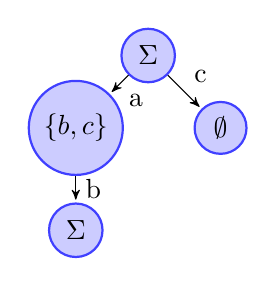
\begin{tikzpicture}[node distance=1.3cm,>=stealth',bend angle=45,auto]
  \tikzstyle{place}=[circle,thick,draw=blue!75,fill=blue!20,minimum size=6mm]
  \tikzstyle{red place}=[place,draw=red!75,fill=red!20]
  \tikzstyle{transition}=[rectangle,thick,draw=black!75,
  			  fill=black!20,minimum size=4mm]
  \tikzstyle{every label}=[red]
  
  \begin{scope}
    \node [place] (w1) {$\Sigma$};
    \node [place] (e1) [below left of=w1] {$\{b,c\}$}
      edge [pre]  node[swap] {a}                 (w1);      
    \node [place] (e2) [below right of=w1] {$\emptyset$}
      edge [pre]  node[swap] {c}                 (w1);      
    \node [place] (e3) [below of=e1] {$\Sigma$}
      edge [pre]  node[swap] {b}                 (e1);      
  \end{scope}
    
\end{tikzpicture}
\caption{Example model.}\label{figure:elSmall}
\end{FIGURE}



We continue with concrete examples.  The model in Figure
\ref{figure:elSmall} satisfies all the following formulae, amongst
others:
\[
\begin{array}{lclclclcl}
\MAY{a} &\qquad&
\MAY{a} \MAY{b} &\qquad&
\MAY{a} \fBang \{b,c\} &\qquad&
\MAY{a} \fBang \{b,c,d\} &\qquad&
\MAY{c} \\[1mm]
\MAY{c} \fBang \{\} &&
\MAY{c} \fBang \{a\} &&
\MAY{c} \fBang \{a,b\} &&
\MAY{a} \land \MAY{c} &&
\MAY{a} (\MAY{b} \land \fBang \{b,c\}
\end{array}
\]

\NI Here we assume, as we do with all subsequent such figures, that
the top note is the root.  The same model does \emph{not} satisfy any
of the following formulae
\[
\MAY{b} \qquad
\fBang \{a\} \qquad
\fBang \{a, c\} \qquad
\MAY{a} \fBang \{b\} \qquad
\MAY{a} \MAY{c} \qquad
\MAY{a} \MAY{b} \fBang \{c\} 
\]

\NI Figure \ref{threemodels} shows various models of $\MAY{a} \MAY{b}$
and Figure \ref{more models} shows one model that does, and one that
does not, satisfy the formula $\fBang \{a,b\}$.  Both models validate
$!\{a, b, c\}$.

\Cathoristic{} does not have the operators $\neg, \lor, $ or $\Rightarrow$.
This has the following two signification consequences.  First, every
satisfiable formula has a unique (up to isomorphism) simplest model.
In Figure \ref{threemodels}, the left model is the unique simplest
model satisfying$\MAY{a} \MAY{b}$.  We will clarify below that model
simplicity is closely related to the process theoretic concept of
similarity, and use the existence of unique simplest models to
construct a \emph{quadratic-time} decision procedure.

\begin{FIGURE}
\centering
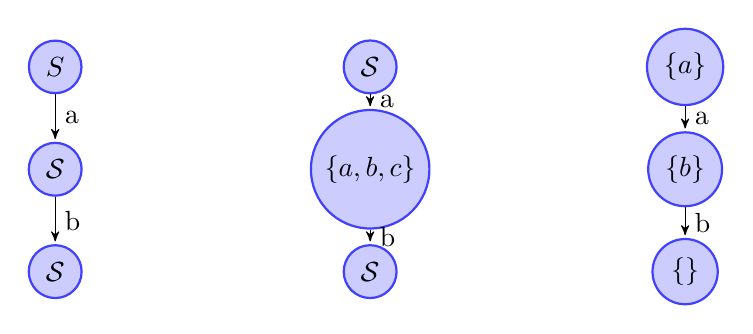
\begin{tikzpicture}[node distance=1.3cm,>=stealth',bend angle=45,auto]
  \tikzstyle{place}=[circle,thick,draw=blue!75,fill=blue!20,minimum size=6mm]
  \tikzstyle{red place}=[place,draw=red!75,fill=red!20]
  \tikzstyle{transition}=[rectangle,thick,draw=black!75,
  			  fill=black!20,minimum size=4mm]
  \tikzstyle{every label}=[red]
  \begin{scope}[xshift=0cm]
    \node [place] (w1) {$S$};
    \node [place] (e1) [below of=w1] {$\mathcal{S}$}
      edge [pre]  node[swap] {a}                 (w1);
    \node [place] (e2) [below of=e1] {$\mathcal{S}$}
      edge [pre]  node[swap] {b}                 (e1);
  \end{scope}   
  \begin{scope}[xshift=4cm]
    \node [place] (w1) {$\mathcal{S}$};
    \node [place] (e1) [below of=w1] {$\{a,b,c\}$}
      edge [pre]  node[swap] {a}                 (w1);
    \node [place] (e2) [below of=e1] {$\mathcal{S}$}
      edge [pre]  node[swap] {b}                 (e1);
  \end{scope}   
  \begin{scope}[xshift=8cm]
    \node [place] (w1) {$\{a\}$};
    \node [place] (e1) [below of=w1] {$\{b\}$}
      edge [pre]  node[swap] {a}                 (w1);
    \node [place] (e2) [below of=e1] {$\{\}$}
      edge [pre]  node[swap] {b}                 (e1);
  \end{scope}   
\end{tikzpicture}
\caption{Various models of $\langle a \rangle \langle b \rangle \top$}
\end{FIGURE}


\begin{FIGURE}
\centering
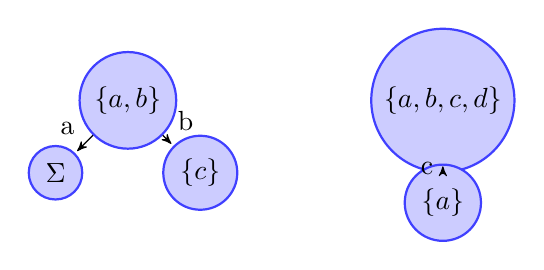
\begin{tikzpicture}[node distance=1.3cm,>=stealth',bend angle=45,auto]
  \tikzstyle{place}=[circle,thick,draw=blue!75,fill=blue!20,minimum size=6mm]
  \tikzstyle{red place}=[place,draw=red!75,fill=red!20]
  \tikzstyle{transition}=[rectangle,thick,draw=black!75,
  			  fill=black!20,minimum size=4mm]
  \tikzstyle{every label}=[red]
  \begin{scope}[xshift=0cm]
    \node [place] (w1) {$\{a, b\}$};
    \node [place] (e1) [below left of=w1] {$\Sigma$}
      edge [pre]  node {a}                 (w1);
    \node [place] (e2) [below right of=w1] {$\{c\}$}
      edge [pre]  node[swap] {b}                 (w1);
  \end{scope}   
  \begin{scope}[xshift=4cm]
    \node [place] (w1) {$\{a, b, c, d\}$};
    \node [place] (e1) [below of=w1] {$\{a\}$}
      edge [pre]  node[swap] {c}                 (w1);
  \end{scope}   
\end{tikzpicture}
\caption{The model on the left validates $!\{a, b, c\}$
while the model on the right does not.}\label{figure:elAndBang:moreMdels}
\end{FIGURE}


Secondly, EL is different from other logics in that there is an
asymmetry between tautologies and contradictories: logics with
conventional negation have an infinite number of non-trivial
tautologies as well as an infinite number of contradictories.  In
contrast, because \cathoristic{} has no negation or disjunction
operator, it is expressively limited in the tautologies it can
express: top and conjunctions of top are its sole tautologies. On the
other hand, the tantum operator, enables an infinite number of
contradictories to be expressed.  For example:
\[
   \MAY{a} \land \fBang \{\} \qquad
   \MAY{a} \land \fBang \{b\} \qquad
   \MAY{a} \land \fBang \{b, c\} \qquad
   \MAY{b} \land \fBang \{\} \qquad
\]


%% \begin{definition} Let $\Gamma$ be an arbitrary set of formulae. We
%% say \emph{$\Gamma$ semantically implies $\phi$}, written $\Gamma
%% \models \phi$, provided for all cathoristic models $\MMM$ if it is the
%% case that $\MMM \models \Gamma$ implies $\MMM \models \phi$.
%% \richard{We do not define $\models \Gamma$ for a set $\Gamma$, only
%% for individual formulae - do we want to change this definition to
%% be of the form $\phi \models \psi$?}  \end{definition}

\NI The semantic consequence relation is standard.\martin{actually
  it's not because the premise can have only one formula. Maybe we
  should elaborate upon this? I think it's intimately related to the
  absence of negation. In classical logic we can use $\Gamma \models
  \phi$ because only a finite bit already implies $ \phi$ and that can
  easily be proven. In EL ... not so much}

\begin{definition} 
 We say the formula $\phi$ \emph{semantically implies} $\psi$, written $\phi
   \models \psi$, provided for all cathoristic models $\MMM$ if it is the
   case that $\MMM \models \phi$ then also $\MMM \models \phi$.
\end{definition}

\begin{example}
\Cathoristic{} shares with other (multi)-modal logics the following
implications:
\begin{eqnarray*}
\MAY{a} \MAY{b} \models \MAY{a} 
 \qquad\qquad
\MAY{a} (\MAY{b} \land \MAY{c}) \models \MAY{a} \MAY{b}
\end{eqnarray*}
As \cathoristic{} is restricted to deterministic models, it also
validates the following formula:
\begin{eqnarray*}
\MAY{a} \MAY{b} \land \MAY{a} \MAY{b}  \models \MAY{a} (\MAY{b} \land \MAY{c})
\end{eqnarray*}
\Cathoristic{} also validates all implications in which the set of constraints is relaxed from left to right. For example:
\begin{eqnarray*}
\fBang \{\} \models \fBang \{a\} 
 \qquad\qquad
\fBang \{\} \models \fBang \{a, b\} 
\end{eqnarray*}
\end{example}


\section{Capturing Inferences Between Atomic Sentences}\label{naturalLanguageInference}

\NI \Cathoristic{} arose as an attempt to answer the question: what is the
simplest logic that can capture inferences between atomic sentences of
natural language?  In this section, we enumerate the sorts of
inferences we are trying to capture.  Then we show how \cathoristic{}
handles these inferences.  Finally, we compare our approach with the
various attempts at expressing the inferences in first-order logic.

\subsection{Intra-Atomic Inferences in Natural Language}

\NI Natural language admits many types of inference between atomic
sentences.  First, exclusion:
\begin{quote}
``Jack is male'' is incompatible with ``Jack is female''
\end{quote}
Second, entailment inferences from dyadic to monadic predicates:
\begin{quote}
``Jack loves Jill'' implies ``Jack loves''
\end{quote}
Third, adverbial inferences:
\begin{quote}
``Jack walks quickly'' implies ``Jack walks''
\end{quote}
Fourth, inferences from conjunctions of sentences to conjunctions of noun-phrases (and vice-versa):
\begin{quote}
``Jack loves Jill'' and ``Jack loves Joan'' together imply that ``Jack loves Jill and Joan''
\end{quote}
Fifth, inferences from conjunctions of sentences to conjunction of predicates\footnote{See \cite{sommers} p.282 for a spirited defence of predicate conjunction against Fregean regimentation.} (and vice-versa):
\begin{quote}
``Jack is bruised'' and ``Jack is humiliated'' together imply that ``Jack is bruised and humiliated''.
\end{quote}

\NI They all can be handled directly and naturally in \cathoristic{}, as we
shall now show.


\subsection{Intra-Atomic Inferences in \Cathoristic{}}
%% We shall show that each of the following inferences can be naturally expressed in \cathoristic{}:
%% \begin{itemize}
%% \item
%% ``Jack is male'' is incompatible with ``Jack is female''
%% \item
%% ``Jack loves Jill'' implies ``Jack loves''\footnote{Although natural languages are full of examples of inferences from dyadic to monadic predicates, there are certain supposed counterexamples to the general rule that a dyadic predicate always implies a monadic one. For example, ``Jack explodes the device'' does not, on its most natural reading, imply that ``Jack explodes''. Our response to cases like this is to distinguish between two distinct monadic predicates $explodes_1$ and $explodes_2$:
%% \begin{itemize}
%% \item
%% $X explodes_1$ iff $X$ is an object that undergoes an explosion
%% \item
%% $X explodes_2$ iff $X$ is an agent that initiates an explosion
%% \end{itemize}
%% Now ``Jack explodes the device'' does imply that ``Jack $explodes_2$'' but does not imply that ``Jack $explodes_1$''. 
%% There is no deep problem here - just another case where natural language overloads the same word in different situation to have different meanings.}
%% \item
%% ``Jack walks quickly'' implies ``Jack walks''
%% \item
%% ``Jack loves Jill'' and ``Jack loves Joan'' together imply that ``Jack loves Jill and Joan''
%% \item
%% ``Jack is bruised'' and ``Jack is humiliated'' together imply that ``Jack is bruised and humiliated''.
%% \end{itemize}

Incompatibility such as that between ``Jack is male'' and ``Jack is
female'' is translated into \cathoristic{} as the pair of incompatible
sentences:
\begin{eqnarray*}
\MAY{jack} \MAY{sex} (\MAY{male} \land \fBang \{male\}) 
   \qquad\qquad
\MAY{jack} \MAY{sex} (\MAY{female} \land \fBang \{female\})
\end{eqnarray*}

\NI Entailment from dyadic to monadic predicates\footnote{Although natural languages are full of examples of inferences from dyadic to monadic predicates, there are certain supposed counterexamples to the general rule that a dyadic predicate always implies a monadic one. For example, ``Jack explodes the device'' does not, on its most natural reading, imply that ``Jack explodes''. Our response to cases like this is to distinguish between two distinct monadic predicates $explodes_1$ and $explodes_2$:
 \begin{itemize}
 \item
 $X explodes_1$ iff $X$ is an object that undergoes an explosion
 \item
 $X explodes_2$ iff $X$ is an agent that initiates an explosion
 \end{itemize}
 Now ``Jack explodes the device'' does imply that ``Jack $explodes_2$'' but does not imply that ``Jack $explodes_1$''. 
There is no deep problem here - just another case where natural language overloads the same word in different situation to have different meanings.}:
``Jack loves Jill'' is translated into \cathoristic{} as:
\begin{eqnarray*}
   \MAY{jack} \MAY{loves} \MAY{jill}
\end{eqnarray*}
The semantics of modalities ensures that this directly entails:
\begin{eqnarray*}
   \MAY{jack} \MAY{loves}
\end{eqnarray*}

\NI Similarly, \cathoristic{} supports inferences from triadic to dyadic
predicates:
\begin{quote}
  ``Jack passed the biscuit to Mary'' implies ``Jack passed the biscuit''
\end{quote}

\NI This can be expressed directly in \cathoristic{} as:
\[
   \MAY{jack} \MAY{passed} \MAY{biscuit} \MAY{to} (\MAY{mary} \land !\{mary\}) \models \MAY{jack} \MAY{passed} \MAY{biscuit}
\]

\NI Adverbial inferences is captures in \cathoristic{} as follows.
\begin{eqnarray*}
\MAY{jack} \MAY{walks} \MAY{quickly}
\end{eqnarray*}
entails:
\begin{eqnarray*}
\MAY{jack} \MAY{walks}
\end{eqnarray*}

\NI \Cathoristic{} directly supports inferences from conjunctions of
sentences to conjunctions of noun-phrases.  As our models are
deterministic, we have the general rule that $ \MAY{a} \MAY{b} \land
\MAY{a} \MAY{c} \models \MAY{a} (\MAY{b} \land \MAY{c})$ from which
it follows that
\begin{eqnarray*}
   \MAY{jack} \MAY{loves} \MAY{jill}
      \qquad\text{and}\qquad
   \MAY{jack} \MAY{loves} \MAY{joan}
\end{eqnarray*}
together imply
\begin{eqnarray*}
\MAY{jack} \MAY{loves} (\MAY{jill} \land \MAY{joan})
\end{eqnarray*}

\NI Using the same rule, we can infer that
\begin{eqnarray*}
   \MAY{jack} \MAY{bruised} \land \MAY{jack} \MAY{humiliated}
\end{eqnarray*}

\NI together imply
\begin{eqnarray*}
\MAY{jack} (\MAY{bruised} \land \MAY{humiliated})
\end{eqnarray*}
 
\subsection{Representing incompatible predicates in \FOL}\label{incompatiblepredicatesinfol}

\NI How are incompatible predicates represented in traditional
\fol{}?  Brachman and Levesque\cite{brachman} introduce the
topic of incompatible predicates by remarking:
\begin{quote}
   We would consider it quite ``obvious'' in this domain that if it
   were asserted that $John$ were a $Man$, then we should answer
   ``no'' to the query $Woman(John)$.
\end{quote}

\NI They propose adding an extra axiom to express the incompatibility:
\[
   \forall x. ( Man(x) \rightarrow \neg Woman(x) )
\]  
 
\NI This proposal imposes an authoring burden on the
knowledge-representer.  We would have to add an extra axiom for every
pair of incompatible predicates.  This proposal becomes particularly
burdensome when dealing with large sets of incompatible predicates.
For example, suppose there are 50 football teams, and a person can
only support one team at a time.  We would need to add $C \cdot {50 \choose 2}$
axioms: incompatibility axioms would become large and unwieldy:
\[
\begin{array}{l}
  \forall x.  \neg (SupportsArsenal(x) \land SupportsLiverpool(x))  \\
  \forall x.  \neg (SupportsArsenal(x) \land SupportsManUtd(x))  \\
  \forall x.  \neg (SupportsLiverpool(x) \land SupportsManUtd(x))  \\
  \qquad \qquad \qquad \vdots
\end{array}
\]

\NI Or, if we treat the football-teams as objects, and have a
two-place $Supports$ relation between people and teams, we could have:
\[
   \forall x, y, z. (Supports(x,y) \land y \neq z \rightarrow \neg Supports(x,z))
\]   

\NI Together with the Unique Names Assumption (which lets us assume
that each football team is distinct from all the others), this
certainly captures the desired uniqueness condition.  But it does so
by using relatively complex logical machinery.

\subsection{Supporting Inferences from Dyadic to Monadic Predicates in Predicate Logic}
If we want to capture the inference from ``Jack loves Jill`` to ``Jack loves'' in \fol{}, we have to add a non-logical axiom:
\[
(\forall x, y) Loves(x,y) \rightarrow Loves(x)
\]

\NI We would have to add an extra non-logical axiom like this for every
n-place predicate.  This is cumbersome at best.  In \cathoristic{}, by
contrast, we do not need to introduce any non-logical machinery at all
to capture these inferences because they all follow from the general
rule that $\MAY{a} \MAY{b} \models \MAY{a}$.

\subsection{Supporting adverbial inferences in \fol{}}

\NI How can we represent verbs in traditional \fol{} so as to
support adverbial inference?  Davidson \cite{davidson2} proposed that
every $n$-place action verb be analysed as an $n$+1-place predicate,
with an additional slot representing an event.  For example, he
analysed ``I flew my spaceship to the Morning Star'' as
\[
\exists x. ( Flew(I, MySpaceship, x) \land To(x, TheMorningStar))
\]
This implies 
\[
\exists x.  Flew(I, MySpaceship, x)
\]
This captures the inference from ``I flew my spaceship to the Morning Star'' to ``I flew my spaceship''.

Predicate Logic cannot support logical inferences between elementary propositions. 
If it is going to support inferences from adverbial sentences, it \emph{cannot} treat them as elementary propositions and must instead \emph{reinterpret} them as logically complex propositions.
The cost of Davidson's proposal is that a seemingly simple sentence, such as ``Jones walks'', turns out on closer inspection not be elementary at all,  but to involve existential quantification:
\[
\exists x.  Walks(Jones, x)
\]

\NI Although Predicate Logic can handle some of these inferences, it
can only do so by reinterpreting the sentences as logically-complex
compound propositions.

\subsection{Summary}
We have looked at various types of inference between atomic
sentences. \Cathoristic{} can handle them directly and naturally.  Traditional
\fol{} has a harder time: it
\emph{can} express incompatibility, but only using complex machinery -
universal quantification, a conditional, negation. \Cathoristic{}, by
contrast, expresses the source of the incompatibility \emph{directly}
using the $!$ operator.  Again, \fol{} \emph{can} express
adverbial inferences, but at the cost of using quantification over
events.  When it comes to inferences from conjunctions of sentences to
conjunctions of noun-phrases (or predicates), \fol{} has
nothing to say because it has no way of expressing conjunctions
between noun-phrases (or predicates) \emph{at all}. In \fol{}, ``Jack is bruised and humiliated'' has to be regimented into
``Jack is bruised and Jack is humiliated''.  This might seem, to the uninitiated, to be the
wrong way around.  

However, \cathoristic{} cannot handle all instances
of sub-propositional inferences.  An example are inferences where the
\emph{subjects} are conjoined such as
\begin{quote}
``Jack loves Jill'' and ``Jim loves Jill'' together imply that ``Jack and Jim love Jill''
\end{quote}

\NI \Cathoristic{} has no way to conjoin noun-phrases in subject-position.

\section{\Cathoristic{} as a language for knowledge representation}\label{kr}


\Cathoristic{} has been used as the representation language for a
large, complex, dynamic multi-agent simulation \cite{evans-and-short}.
This is an industrial-sized application, involving tens of thousands
of rules and facts\footnote{The application has thousands of paying
  users, and available for download on the App Store for the iPad
  \cite{Versu}.}.  In this simulation, the entire world state is stored
as a set of \cathoristic{} formulae - all other aspects of world state
are transient and computed as needed.  The current true sentences are
represented in a cathoristic model.\martin{THis is inconsistent: are the facts stored as CL formulae or a CL model?}

We shall first sketch how facts are represented, before describing some
advantages of \cathoristic{} over a more traditional \fol{}
representation of knowledge.

\subsection{Representing facts  in \cathoristic{}}

A sentence involving a one-place predicate of the form $p(a)$ is
expressed in \cathoristic{} as
\begin{eqnarray*}
   \MAY{a} \MAY{p}.
\end{eqnarray*}

\NI A sentence involving a many-to-many two-place relation of the form
$r(a,b)$ is expressed in \cathoristic{} as
\begin{eqnarray*}
  \MAY{a} \MAY{r} \MAY{b}.
\end{eqnarray*}

\NI But a sentence involving a many-to-one two-place relation of the
form $r(a,b)$ is expressed as:
\begin{eqnarray*}
  \MAY{a} \MAY{r} (\MAY{b} \land \fBang \{b\}).
\end{eqnarray*}

\NI The translation is detailed in Section \ref{translationFOLtoFOEL}.

So, for example, to say that ``Jack likes Jill'' (where ``likes'' is,
of course, a many-many relation), we would write:
\begin{eqnarray*}
  \MAY{jack} \MAY{likes} \MAY{jill}.
\end{eqnarray*}

\NI But to say that ``Jack is married to Joan''
(where``is-married-to'' is a many-one relation), we would write:
\begin{eqnarray*}
  \MAY{jack} \MAY{married} (\MAY{joan} \land \fBang \{joan\}).
\end{eqnarray*}

\NI Colloquially, we might say that ``Jack is married to Joan - and
only Joan''.  Note that the relations are placed in infix position, so
that the facts about an object are ``contained'' within the object.
One reason for this particular way of structuring the data will be
explained below.
 
\martin{ I think the rest of this section could be structured more
  clearly. I think we are saying CL is good for the following two
  (very different) reasons.  (1) Convenience of representation for
  humans. (2) Algorithmic properties, which are about (a) efficient
  model update and (b) efficient queries. CL is good regarding (2)
  because formulae have tree structure and trees can be efficiently
  represented using pointers manipulated using lot's of well-known
  algorithms. Maybe state the general picture first and then give
  examples?}

Consider the following facts about a gentleman named Brown:

\[
   \MAY{brown} 
   \left(
   \begin{array}{l}
     \MAY{sex} (\MAY{male} \land \fBang \{male\}) \\
        \qquad \AND \\
     \MAY{friends} (\MAY{lucy} \land \MAY{elizabeth}) 
   \end{array}
   \right)
\]

\NI All facts  starting with the prefix $\MAY{brown}$ form a
sub-tree of the entire database.  And all  facts which start with
the prefix $\MAY{brown} \MAY{friends}$ form a sub-tree of that tree.
A sub-tree can be treated as an individual via its prefix.  
A sub-tree of formulae is the \cathoristic{} equivalent of an
\emph{object} in an object-oriented programming language.

To model change over time, we assert and retract statements from the
database, using a non-monotonic update mechanism.  If a fact is
inserted into the database that involves a state-labelling restricting
the permissible  transitions emanating from that state, then all
transitions out of that state that are incompatible with the
restriction are removed.  So, for example, if the database currently
contains the fact that the traffic light is amber, and then we update
the database to assert the traffic light is red:
\[
\MAY{tl} \MAY{colour} (\MAY{red} \land !\{red\})
\]
Now the restriction on the state (that red is the only transition)
means that the previous transition from that state (the transition
labelled with amber) is automatically removed.

The tree-structure of formulae allows us to express the \emph{life-time of data} in a natural way. 
If we wish a piece of data $d$ to exist for just the duration of a proposition $t$, then we make $t$ be a sub-expression of $d$. 
For example, if we want the friendships of an agent to exist just as long as the agent, then we place the relationships inside the agent: 
\[
\MAY{brown} \MAY{friends}
\]
Now, when we remove $\MAY{brown}$ all the sub-trees, including the data about who he is friends with, will be automatically deleted as well.

Another advantage of our representation is that we get a form of \emph{automatic currying} which simplifies queries.
So if, for example, Brown is married to Elizabeth, then the database would contain 
\begin{eqnarray*}
\MAY{brown} \MAY{married} (\MAY{elizabeth} \land \fBang \{elizabeth\})
\end{eqnarray*}
In \cathoristic{}, if we want to find out whether Brown is married, we can query the sub-formula directly -  we just ask if 
\begin{eqnarray*}
\MAY{brown} \MAY{married}
\end{eqnarray*}
In \fol, if $married$ is a two-place predicate, then we need to fill in the extra argument place with a free variable - we would need to find out if there exists an $X$ such that $married(brown, X)$ - this is slower to compute and more cumbersome to type. 

\subsection{Simpler postconditions}

In this section, we contrast the representation in action languages based on \fol{}\footnote{E.g. STRIPS \cite{strips}}, with our \cathoristic{}-based representation.
Action definitions are rendered in typewriter font.

When expressing the pre- and post-conditions of an action, planners
based on \fol{} have to explicitly describe the propositions that
are removed when an action is performed:
\begin{verbatim}
   action move(A, X, Y)
       preconditions
           at(A, X)
       postconditions
           add: at(A, Y) 
           remove: at(A, X)
\end{verbatim}
Here, we need to explicitly state that when $A$ moves from $X$ to $Y$, $A$ is no longer at $X$. It might seem obvious to us that if $A$ is now at $Y$, he is no longer at $X$ - but we need to explicitly tell the system this. This is unnecessary, cumbersome and error-prone. In \cathoristic{}, by contrast, the exclusion operator means we do not need to specify the facts that are no longer true:
\begin{verbatim}
   action move (A, X, Y)
       preconditions
           <A><at>(<X> /\ !{X})
       postconditions
           add: <A><at>(<Y> /\ !{Y})
\end{verbatim}
The tantum operator $!$ makes it clear that something can only be at one
place at a time, and the non-monotonic update rule described above
\emph{automatically} removes the old invalid location data.

\subsection{Using tantum $!$  to optimise preconditions}
\label{optimizingpreconditions}
Suppose, for example, we want to find all married couples who are both Welsh.
In Prolog, we might write something like:
\begin{verbatim}
   welsh_married_couple(X, Y) :-
       welsh(X),
       welsh(Y),
       spouse(X,Y).
\end{verbatim}	
Rules like this create a large search-space because we need to find all instances of $welsh(X)$ and all instances of  $welsh(Y)$ and take the cross-product \cite{smith-and-genesereth}. If there are $n$ Welsh people, then we will be searching $n^2$ instances of $(X,Y)$ substitutions.

If we express the rule in \cathoristic{}, the compiler is able to use the extra information expressed in the $!$ operator to reorder the literals to find the result significantly faster.
Assuming someone can only have a single spouse at any moment, the rule is expressed in \cathoristic{} as:
\begin{verbatim}
   welsh_married_couple(X, Y) :-
       <welsh> <X>,
       <welsh> <Y>,
       <spouse> <X> (<Y> /\ !{Y}).
\end{verbatim}	
Now the compiler is able to reorder these literals to minimize the search-space. 
It can see that, once $X$ is instantiated, the following literal can be instantiated without increasing the search-space:
\begin{verbatim}
   <spouse> <X> (<Y> /\ !{Y})
\end{verbatim}
The \emph{tantum} operator can be used by the compiler to see that there is at most one $Y$ who is the spouse of $X$.
So the compiler reorders the clauses to produce:
\begin{verbatim}
   welsh_married_couple (X, Y) :-
       <welsh> <X>,
       <spouse> <X> (<Y> /\ !{Y}),
       <welsh> <Y>.
\end{verbatim}	
Now it is able to find all results by just searching $n$ instances - a significant optimization.
In our application, this optimisation has made a significant difference to the run-time cost of query evaluation.







\section{Related Work}

\subsection{Brandom's Incompatibility Semantics}
In \cite{brandom2} and \cite{brandom}, Brandom has emphasised that logical negation is a degenerate case of material incompatibility:
\begin{quote}
Incompatible sentences are Aristotelian \emph{contraries}. A sentence and its negation are \emph{contradictories}. What is the relation between these? Well, the contradictory is a contrary: any sentence is incompatible with its negation. What distinguishes the contradictory of a sentence  from all the rest of its contraries? The contradictory is the \emph{minimal} contrary: the one that is entailed by all the rest. Thus every contrary of ``Plane figure $f$ is a circle'' - for instance ``$f$ is a triangle'', ``$f$ is an octagon'', and so on - entails ``$f$ is \emph{not} a circle''.
\end{quote}
In \cite{brandom}, Chapter 5, Appendix I, Brandom developed a new type of semantics, Incompatibility Semantics, that takes material incompatibility - rather than truth-assignment - as the semantically primitive notion.

Incompatibility Semantics applies to any language, $\mathcal{L}$, given as a set of sentences. 
It uses an incompatibility function $\mathcal{I}$, that, given a set of sentences $S \subseteq \mathcal{L}$, produces the set of sets of sentences that are incompatible with $S$.
We assume that $\mathcal{I}$ satisfies the monotonicity requirement (Brandom calls it ``Persistence''):
\[
\text{If } X \in \mathcal{I}(Y) \text{ and } X \subseteq X' \text{ then } X' \in \mathcal{I}(Y)
\]
Now Brandom defines entailment in terms of the incompatiblity function. Given a set $X \subseteq \mathcal{L}$ and an individual sentence $\phi \in \mathcal{L}$:
\[
X \models \phi \text{ iff } \mathcal{I}(\{\phi\}) \subseteq \mathcal{I}(X)
\]
Now, given material incompatibility (as captured by the $\mathcal{I}$ function) and entailment, he introduces logical negation as a \emph{derived} concept. Using $N \phi$ for the negation of $\phi$, he introduces negation via the rule:
\[
\{N \phi\} \in \mathcal{I}(X) \text{ iff } X \models \phi
\]
Brandom goes on to show that the $N$ operator, as defined, satisfies the laws of classical negation. 
He also introduces a modal operator, again defined in terms of material incompatibility, and shows that this operator satisfies the laws of $S5$.

\ELFULL{} was inspired by Brandom's vision that material incompatibility is conceptually prior to logical negation:
in other words, it is possible for a community of language users to deploy a language including a material incompatibility relation, even if that language has no explicit logical operators such as negation.
The language users of this simple language may go on to introduce logical operators, in order to make certain inferential properties explicit - but this is an optional further development. 
The language before that addition was already in order as it is.

The approach taken in this paper takes Brandom's original insight in a different direction.
While Brandom defines an unusual (non truth-conditional) semantics that applies to any language, we have defined a unusual logic with a standard (truth-conditional) semantics.






\subsection{Other Related work}

Linguists have also investigated how mutually exclusive alternatives
are expressed \cite{OKeeffeA:rouhanocl}\martin{See John C email for
  more precise reference}, but, to the best of our knowledge have not
proposed formal theories of linguistic exclusion.

Linear logic \cite{GirardJY:linlog,GirardJY:protyp} is a refinement of
first-order logic and was introduced by J.-Y.~Girard with the aim of
bringing the symmetries of classical logic to constructive
logic. Linear logic has been fruitful in a variety of fields, in
particular in the study of typing systems, where the concept of
linearity puts type-based resource handling on a sound logical basis.

Linear logic splits conjunction into two: additive and multiplicative
conjunction The former, additive conjunction $A \& B$, is especially
interesting in the context of \ELFULL{}. It can be interpreted
\cite{AbramskyS:comintoll} as an external choice operation in the
terminology of CSP \cite{HoareC:comseq}. External, because the choice
is offered to the environment.  This interpretation has been
influential in the study of types for process calculus,
e.g.~\cite{HondaK:unitypsfsifLONG,TakeuchiK:intbaslaits,HondaK:lanpriatdfscbp}.
Implicitly, additive conjunction gives an explicit upper bound on how
many different options the environment can choose from. For example in
$A \& B \& C$ we have three options (assuming that none of $A, B, C$
can be decomposed into further additive conjunctions).  With this in
mind, and simplifying a great deal, a key difference between $!A$ and
additive conjunction $A \& B$ is that the individual actions in $!A$
have no continuation, while they do with $A \& B$: $!\{l, r\}$ says
that at this point the only available actions are $l$ and $r$. What
happens at later states is not constraind by $!A$.  In contrast, $A \&
B$ says not only that at this point the only available options are $A$
and $B$, but also that if we choose $A$, then $A$ holds 'for ever',
and likewise for choosing $B$. To be sure, the alternatives in $A \&
B$ may themselves contain further additive conjunctions, and in this
way express how exclusion changes 'over time'.

In summary, \ELABR{} and linear logic offer an operator that restricts
the available options. How are they related? Linear logic has an
explicit linear negation $(\cdot)^{\bot}$ which, unlike classical
negation, is constructive. In constrast, \ELABR{} defines a restricted
form negation from $!A$. Can these two perspectives be frutifully
reconciled?

In this context it is also worth noting that like eremic logic, linear
logic has been used for logic programming
\cite{HodasJS:logproiafoill,WinikoffMD:logprowll,PymDJ:uniprotiollp,HarlandJ:prolygao,MillerD:surlinlp}
and as a programming language for narrative generation
\cite{BosserAG:linlogpfng}, see references therein.

Another formalism that has a form of explicit description of mutually
exclusive option as a core primitive are process calculi. They are
models of computation based on the idea of message passing between
actors running in parallel. Labelled transition systems are often used
as models for process calculi, and many concepts, for example
bisimulations and Hennessy-Milner logic, used for developing eremic
logic originated from process theory (although some, such as
bisimulation, evolved independently in other contexts).

Process calculi traditionally have sums, which, in their most general
form, are:
\[
     \sum_{i \in I} P_i
\]
That is a process that can internally choose, or be chosen to evolve
into the process $P_i$ for each $i$. Once the choice is made, all
other options disappear.  Usually, so much generality is not
considered. Instead, input-guarded sums are much better behaved (and
strictly less expressive):
  \[
     \sum_{i \in I} x_{i}(v_i)P_i
  \]
This is a process that can receive a message on each channel $x_i$
and, if such a message arrives with payload $y$, evolve into
$P_i{y/v_i}$ which is the process obtained from $P_i$ by substituting
$y$ for the bound variable $v_i$.  An even better behaved process is
obtained if all inputs use the same input channel and we have only
finitely many alternatives:
  \[
     \sum_{i = 1}^n x(v)P_i
  \]
  Simplifying a great deal, this can be seen as a proof for linear
  logic's additive conjunction
  \[
     \&_{i = 1}^n x(v)A_i
  \]
  provided each $P_i$ is a proof of $A_i$.  It is possible to extend
  the Curry-Howard correspondence to (fragments of) linear logic on
  one side and process calculi on the other \cite{GaySJ:typcalosp}.

In this way, process calculi are related to linear logic (by using
formulae as types) and to eremic logic (because processes and eremic
formulae can be modelled by labelled transition systems, and because
eremic logic is close to logics for processes).\martin{rephrase. How
  did process theory influence EL?}




% \section{Conclusion}\label{conclusion}

We have introduced \Cathoristic{} as a system for capturing logical inferences between the \emph{atomic} sentences of natural language.
Now there have been various attempts to capture these inferences by translating into \fol{}.
We have argued that our translation into \Cathoristic{} is more efficient and more ergonomic, because we are translating into a simple propositional logic - rather than a complex quantificational logic.
We have used \Cathoristic{} as the basis for a logic-programming language that has served in an industrial AI application.

%We thank Marek Sergot, Tom Smith, and Giacomo Turbanti for their thoughtful comments.


\bibliography{../bib} 

\section{Inference Rules}\label{elAndBangMore}

\begin{FIGURE}
\begin{RULES}

  \ZEROPREMISERULENAMEDRIGHT
  {
    \phi \judge \phi
  }{Id}
    \qquad
  \ZEROPREMISERULENAMEDRIGHT
  {
    \phi \judge \top
  }{$\top$-Right}
    \qquad
  \ZEROPREMISERULENAMEDRIGHT
  {
    \bot \judge \phi
  }{$\bot$-Left}
    \qquad
  \TWOPREMISERULENAMEDRIGHT
  {
    \phi \judge \psi
  }
  {
    \psi \judge \xi
  }
  {
    \phi \judge \xi
  }{Trans}
    \\\\
  \ONEPREMISERULENAMEDRIGHT
  {
    \phi \judge \psi
  }
  {
    \phi \AND \xi \judge \psi
  }{$\AND$-Left 1}
     \qquad
  \ONEPREMISERULENAMEDRIGHT
  {
    \phi \judge \psi
  }
  {
    \xi \AND \phi  \judge \psi
  }{$\AND$-Left 2}
     \qquad
  \TWOPREMISERULENAMEDRIGHT
  {
    \phi \judge \psi
  }
  {
    \phi \judge \xi
  }
  {
    \phi \judge \psi \AND \xi
  }{$\AND$-Right}
     \\\\
     \ONEPREMISERULENAMEDRIGHT
     {
       a \notin A
     }
     {
       !A \AND \MAY{a}{\phi} \judge \bot
     }{$\bot$-Right 1}
        \qquad
     \ZEROPREMISERULENAMEDRIGHT
     {
       \MAY{a}{\bot} \judge \bot
     }{$\bot$-Right 2}
     \qquad
     \TWOPREMISERULENAMEDRIGHT
     {
       \phi \judge !A
     }
     {
       A \subseteq A'
     }
     {
       \phi \judge!A'
     }{!-Right 1}
     \\\\
     \TWOPREMISERULENAMEDRIGHT
     {
       \phi \judge !A
     }
     {
       \phi \judge !B
     }
     {
       \phi \judge !(A \cap B)
     }{!-Right 2}
     \qquad
     \ONEPREMISERULENAMEDRIGHT
     {
       \phi \judge \psi
     }
     {
       \MAY{a}{\phi} \judge \MAY{a}{\psi}
     }{Normal}
     \qquad
     \ONEPREMISERULENAMEDRIGHT
     {
       \phi \judge \MAY{a}\psi \land \MAY{a}\xi
     }
     {
       \phi \judge \MAY{a}(\psi \land \xi)
     }{Det}
\end{RULES}
\caption{Proof rules.}\label{figure:elAndBangRules}
\end{FIGURE}


\NI We now present the inference rules for \cathoristic{}. There are no
axioms.

\begin{definition} Judgements are of the following form.
\[
  \phi \judge \psi.
\]
We also write $\judge \phi$ as a shorthand for $\top \judge
\phi$. Figure \ref{figure:elAndBangRules}
presents all proof rules.
\end{definition}

\NI Note that $\phi$ and $\psi$ are single formulae, not sequents.  By
using single formulae, we can avoid structural inference rules.  The
proof rules can be grouped in two parts: standard rules and rules
unique to \cathoristic{}.  Standard rules are [\RULENAME{Id}],
[\RULENAME{$\top$-Right}], [\RULENAME{$\bot$-Left}],
[\RULENAME{Trans}], [\RULENAME{$\AND$-Left 1}],
[\RULENAME{$\AND$-Left 2}] and [\RULENAME{$\AND$-Right}]. They hardly need
explanation as they are variants of familiar rules for propositional
logic, see e.g.~\cite{TroelstraAS:basprot,vanDalenD:logstr}.  We now
explain the rules that give \cathoristic{} its distinctive properties.

The rule [\RULENAME{$\bot$-Right 1}]  captures the core
exclusion property of the tantum !: for example if $A = \{male, female\}$
then $\MAY{orange}{\phi}$ is incompatible with $!A$. Thus $!A \AND
\MAY{orange}{\phi}$ must be false.

The rule [\RULENAME{$\bot$-Right 2}] expresses that falsity is `global'
  and cannot be suppressed by the modalities. For example
  $\MAY{orange}{\bot}$ is false, simply because $\bot$ is already
  false.

[\RULENAME{Normal}] enables us to prefix an inference with a
may-modality.  This rule can also be stated in the the following more
general form:
\[
   \ONEPREMISERULENAMEDRIGHT
   {
     \phi_1\AND ...\AND \phi_n \judge \psi
   }
   {
     \MAY{a}{\phi_1}\AND ...\AND \MAY{a}{\phi_n} \judge \MAY{a}{\psi}
   }{Normal-Multi}
\]

\NI But it is not necessary because [\RULENAME{Normal-Multi}] is
derivable from [\RULENAME{Normal}] as we show in the examples below.

%% \subsection{Example inferences}

%% \NI We prove that we can use $\phi \AND \psi \judge \xi$ to derive
%% $\MAY{a} \phi \land \MAY{a} \psi \judge \MAY{a} \xi$:

%% \begin{center}
%%   \AxiomC{$\MAY{a} \phi \land \MAY{a} \psi \judge \MAY{a} \phi \land \MAY{a} \psi$}
%%   \RightLabel{\RULENAME{\small Det}}
%%   \UnaryInfC{$\MAY{a} \phi \land \MAY{a} \psi \judge \MAY{a} (\phi \land \psi)$}
%%   \AxiomC{$\phi \AND \psi  \judge  \xi$}
%%   \RightLabel{\RULENAME{\small Normal}}
%%   \UnaryInfC{$\MAY{a} (\phi \AND \psi)  \judge  \MAY{a} \xi$}
%%   \RightLabel{\RULENAME{\small Trans}}
%%   \BinaryInfC{$\MAY{a} \phi \land \MAY{a} \psi \judge \MAY{a} \xi$}
%%   \DisplayProof
%% \end{center}


%% \NI Figure \ref{figure:elAndBangMore:bigDerivations} demonstrates how
%% to infer $\MAY{a}!\{b,c\} \land \MAY{a}!\{c,d\} \judge \MAY{a}!\{c\}$
%% and $\MAY{a} !\{b\} \land \MAY{a} \MAY{c} \top \judge \MAY{d} \top$.

\subsection{\RULENAME{!-Left} and \RULENAME{!-Right}}

The rules [\RULENAME{!-Right 1}, \RULENAME{!-Right 2}] jointly express
how the subset relation $\subseteq$ on sets of actions relates to
provability. Why  don't we need a corresponding rule \RULENAME{!-Left} for
strengthening $!$ on the left hand side?
\[
   \TWOPREMISERULENAMEDRIGHT
     {
       \phi \AND \, !A \judge \psi
     }
     {
       A' \subseteq A
     }
     {
       \phi \AND\, !A' \judge \psi
     }{!-Left}
\]
The reason is that [\RULENAME{!-Left}] can be derived as follows.
\begin{center}
  \AxiomC{$\phi \AND\, !A'  \judge  \phi \AND\, !A'$}
  \AxiomC{$A' \subseteq A$}
  \RightLabel{\small\RULENAME{!-Right 1}}
  \BinaryInfC{$\phi \AND\, !A'  \judge  \phi \AND\, !A$}
  \AxiomC{$\phi \AND\, !A  \judge  \psi$}
  \RightLabel{\small\RULENAME{Trans}}
  \BinaryInfC{$\phi \AND\, !A'  \judge  \psi$}
  \DisplayProof
\end{center}

\NI Readers familiar with object-oriented programming will recognise
[\RULENAME{!-Left}] as contravariant and [\RULENAME{!-Right 1}]
as covariant subtyping. Honda \cite{HondaK:thetypftpc} develops a full
theory of subtyping based on similar ideas.  All three rules embody
the intuition that whenever $A \subseteq A'$ then asserting that $!A'$
is as strong as, or a stronger statement than
$!A$. [\RULENAME{!-Left}] simply states that we can always strengthen
our premise, while [\RULENAME{!-right 1}] allows us to weaken the
conclusion.

%% \subsection{Characteristic formulae}

%% In order to prove completeness, below, we need the notion of a
%% \emph{characteristic formula} of a model.  The function
%% $\SIMPL{\cdot}$ takes a formula as argument and returns
%% the least upper bound of the satisfying models. Characteristic formulae go the other way: given a model
%% $\MMM$, $\CHAR{\MMM}$ is the logically weakest formula that describes that model. 
%% %\clearpage
%% %\begin{SIDEWAYSFIGURE}

\begin{center}
  \AxiomC{$!\{b,c\} \judge !\{b,c\}$}
  \RightLabel{\small \RULENAME{ $\land$ Left 1}}
  \UnaryInfC{$!\{b,c\} \land !\{c,d\} \judge !\{b,c\}$}
  \AxiomC{$!\{c,d\} \judge !\{c,d\}$}
  \RightLabel{\small \RULENAME{ $\land$ Left 2}}
  \UnaryInfC{$!\{b,c\} \land !\{c,d\} \judge !\{c,d\}$}
  \RightLabel{\small \RULENAME{ ! Right 2}}
  \BinaryInfC{$!\{b,c\} \land !\{c,d\} \judge !\{c\}$}
  \RightLabel{\small \RULENAME{ Normal}}
  \UnaryInfC{$\MAY{a} (!\{b,c\} \land !\{c,d\}) \judge \MAY{a} !\{c\}$}
  \AxiomC{$\MAY{a} !\{b,c\} \land \MAY{a} !\{c,d\} \judge \MAY{a} !\{b,c\} \land \MAY{a} !\{c,d\}$}
  \RightLabel{\small \RULENAME{ Det}}
  \UnaryInfC{$\MAY{a} !\{b,c\} \land \MAY{a} !\{c,d\} \judge \MAY{a} (!\{b,c\} \land !\{c,d\})$}
  \RightLabel{\small \RULENAME{ Trans}}
  \BinaryInfC{$\MAY{a} !\{b,c\} \land \MAY{a} !\{c,d\} \judge \MAY{a}!\{c\}$}
  \DisplayProof
\end{center}
\vspace{7mm}
\begin{center}
  \AxiomC{$!\{b\} \land \MAY{c}\top \judge \bot$}
  \RightLabel{\small \RULENAME{ Normal}}
  \UnaryInfC{$\MAY{a}(!\{b\} \land \MAY{c}\top) \judge \MAY{a} \bot$}
  \AxiomC{$\MAY{a}!\{b\} \land \MAY{a} \MAY{c}\top \judge \MAY{a}!\{b\} \land \MAY{a} \MAY{c}\top$}
  \RightLabel{\small \RULENAME{ Det}}
  \UnaryInfC{$\MAY{a}!\{b\} \land \MAY{a} \MAY{c}\top \judge \MAY{a}(!\{b\} \land \MAY{c}\top)$}
  \RightLabel{\small \RULENAME{ Trans}}
  \BinaryInfC{$\MAY{a}!\{b\} \land \MAY{a} \MAY{c}\top  \judge \MAY{a} \bot$}  
  \AxiomC{$\MAY{a}\bot \judge \bot$}
  \RightLabel{\small \RULENAME{ Trans}}
  \BinaryInfC{$\MAY{a}!\{b\} \land \MAY{a} \MAY{c}\top  \judge \bot$}  
  \AxiomC{$\bot \judge \MAY{d} \top$}
  \RightLabel{\small \RULENAME{ Trans}}
  \BinaryInfC{$\MAY{a}!\{b\} \land \MAY{a} \MAY{c}\top  \judge  \MAY{d} \top$}    
  \DisplayProof
\end{center}

\caption{Derivations of $\MAY{a}!\{b,c\} \land \MAY{a}!\{c,d\} \judge \MAY{a}!\{c\}$ (top) and
 $\MAY{a} !\{b\} \land \MAY{a} \MAY{c} \top \judge \MAY{d} \top$ (bottom).}\label{figure:elAndBangMore:bigDerivations}
\end{SIDEWAYSFIGURE}

%% %clearpage

%% \begin{definition}
%% Let $\MMM$ be a cathoristic model that is a tree.
%% \begin{eqnarray*}
%%   \CHAR{\bot} &\ =\ & \langle a \rangle \top \AND ! \emptyset  \mbox{ for some fixed action }a \in \Sigma  \\
%%   \CHAR{\MMM, w} & = & \mathsf{bang}(\MMM,w) \AND \bigwedge_{w \xrightarrow{a} w'} \langle a \rangle \CHAR{\MMM, w'}  
%% \end{eqnarray*}

%% \end{definition}

%% \NI Note that $\bot$ requires a particular action $a \in \Sigma$. This
%% is why we required, in Section \ref{elsyntax}, that $\Sigma$ is
%% non-empty.

%% The functions $\mathsf{bang}(\cdot)$ on models are given by the
%% following clauses.

%% \begin{eqnarray*}
%%   \mathsf{bang}((S,\rightarrow,\lambda),w) 
%%      & \ = \ & 
%%   \begin{cases}
%%     \top & \mbox{ if } \lambda(w) = \Sigma  \\
%%     ! \; \lambda(w) & \mbox{ otherwise }  
%%   \end{cases} \\
%% \end{eqnarray*}

%% \NI Note that $\CHAR{\MMM}$ is finite if $\MMM$ contains no cycles and
%% if $\lambda(x)$ is either $\Sigma$ or finite for all states $x$.  We
%% state without proof that $\SIMPL{\cdot}$ and $\CHAR{\cdot}$ are
%% inverses of each other (for tree models $\MMM$) in that:

%% \begin{itemize}

%% \item $\SIMPL{\CHAR{\MMM}} \ \MODELEQ \  \MMM$. 

%% \item $\models \CHAR{\SIMPL{\phi}}$ iff $\models\phi$.

%% \end{itemize}


\subsection{Soundness and completeness}

\begin{theorem}\label{theorem:elAndBang:soundComplete}
The rules in Figure \ref{figure:elAndBangRules} are sound and complete:
\begin{enumerate}

\item\label{theorem:elAndBang:sound} (Soundness) $\phi \judge \psi$ implies $\phi \models \psi$.

\item\label{theorem:elAndBang:complete} (Completeness) $\phi \models \psi$ implies $\phi \judge \psi$.

\end{enumerate}
\end{theorem}

%% \NI Soundness is immediate from the definitions. 
%%  To prove completeness  we will show that $\phi
%% \models \psi$ implies there is a derivation of $\phi \judge \psi$.  Our proof
%% will make use of two key facts (proved in Sections \ref{prooflemma4} and \ref{prooflemma5} below):

%% %% \begin{definition}
%% %% Let $\Gamma$ be an arbitrary set of eremic formulae. We write $\MMM
%% %% \models \Gamma$ provided $\MMM \models \phi$ for all $\phi \in
%% %% \Gamma$.  We write $\Gamma \models \phi$ if for all eremic models
%% %% $\MMM$ $\MMM \models \Gamma$ implies $\MMM \models \phi$.  We write
%% %% $\phi_1, ..., \phi_n \judge \psi$ whenever $\BIGAND_{i}\phi_i \judge
%% %% \psi$.  For arbitrary sets $\Gamma$ of formulae, we write $\Gamma
%% %% \judge \psi$ provided there are $\phi_1, ..., \phi_n \in \Gamma$ such
%% %% that $\phi_1, ..., \phi_n \judge \psi$.
%% %% \end{definition}

%% %% \begin{corollary}
%% %% The rules in Figure \ref{figure:elAndBangRules} are sound and complete:
%% %% \begin{enumerate}

%% %% \item(Soundness) $\Gamma \judge \psi$ implies $\Gamma \models \psi$.

%% %% \item (Completeness) $\Gamma \models \psi$ implies $\Gamma \judge \psi$. 

%% %% \end{enumerate}
%% %% \end{corollary}

%% %% \begin{proof}
%% %% For soundness assume that $\MMM$ is a model with $\MMM \models
%% %% \Gamma$.  We know that $\Gamma \judge \psi$ means that we can find a
%% %% finite number of formulae $\phi_i \in \Gamma$ with $\AND_i \phi \judge
%% %% \psi$.  By soundness then also $\AND_i \phi \models \psi$, hence
%% %% clearly $\Gamma \models \psi$.


%% \begin{lemma}\label{lemma:completeness:4}
%% If $\MMM \models \phi$ then $\CHAR{\MMM} \judge \phi$.
%% \end{lemma}

%% \begin{lemma}\label{lemma:completeness:5}
%% For all formulae $\phi$, we can derive $\phi \judge \CHAR{\SIMPL{\phi}}$.
%% \end{lemma}

%% \NI Lemma \ref{lemma:completeness:4} states that, if $\phi$ is
%% satisfied by a model, then there is a proof that the characteristic
%% formula describing that model entails $\phi$.  In Lemma
%% \ref{lemma:completeness:5}, $\SIMPL{\phi}$ is the simplest
%% model satisfying $\phi$, and $\CHAR{\MMM}$ is the simplest formula
%% describing $m$, so $\CHAR{\SIMPL{\phi}}$ is a simplified form of
%% $\phi$. This lemma states that \cathoristic\ has the inferential capacity to
%% transform any proposition into its simplified form.

%% With these two lemmas in hand, the proof of completeness is
%% straightforward.  Assume $\phi \models \psi$.  Then all models which satisfy
%% $\phi$ also satisfy $\psi$.  In particular, $\SIMPL{\phi} \models \psi$.  Then
%% $\CHAR{\SIMPL{\phi}} \judge \psi$ by Lemma \ref{lemma:completeness:4}.  But we
%% also have, by Lemma \ref{lemma:completeness:5}, $\phi \judge
%% \CHAR{\SIMPL{\phi}} $.  So by transitivity, we have $\phi \judge \psi$.  

%% \subsection{Proofs of Lemmas \ref{lemma:completeness:4}, \ref{lemma:completeness:5} and \ref{final_completeness_lemma}}

%% \subsubsection{Proof of Lemma \ref{lemma:completeness:4}}
%% \label{prooflemma4}
%% If $\MMM\models \phi$ then $\CHAR{\MMM} \judge \phi$.

%% \NI We proceed by induction on $\phi$.

%% %\setcounter{mycase}{0}

%% \CASE{$\phi$ is $\top$} Then we can prove $ \CHAR{\MMM} \judge \phi$
%% immediately using axiom [\RULENAME{$\top$ Right}.

%% \CASE{$\phi$ is $\psi \AND \psi'$} By the induction hypothesis, $
%% \CHAR{\MMM} \judge \psi$ and $ \CHAR{\MMM} \judge \psi'$.  The proof
%% of $ \CHAR{\MMM} \judge \psi \AND \psi'$ follows immediately using
%% [\RULENAME{$\AND$ Right}.

%% \CASE{$\phi$ is $\langle a \rangle \psi$}
%% If $\MMM \models \langle a \rangle \psi$, then either $\MMM = \bot$ or $\MMM$ is a  model of the form $(\CAL{L},w)$.

%% \SUBCASE{$\MMM = \bot$} In this case, $ \CHAR{\MMM} = \CHAR{\bot} =
%% \bot$. (Recall, that we are overloading $\bot$ to mean both the model
%% at the bottom of our lattice and a formula (such as $\langle a \rangle
%% \top \AND !\emptyset$) which is always false).  In this case, $ \CHAR{\bot}
%% \judge \langle a \rangle \psi$ using [\RULENAME{$\bot$ Left}.

%% \SUBCASE{$m$ is a model of the form $(\CAL{L},w)$} Given $\MMM \models
%% \langle a \rangle \psi$, and that $\MMM$ is a model of the form
%% $(\CAL{L},w)$, we know that:
%% \[
%% (\CAL{L},w) \models \langle a \rangle \psi
%% \]
%% From the satisfaction clause for $\langle a \rangle$, it follows that:
%% \[
%% \exists w' \mbox{ such that } w \xrightarrow{a} w' \mbox { and } (\CAL{L},w') \models \psi
%% \]
%% By the induction hypothesis:
%% \[
%%  \CHAR{(\CAL{L},w')} \judge \psi
%% \]
%% Now by [\RULENAME{Normal}]:
%% \[
%% \langle a \rangle  \CHAR{(\CAL{L},w')} \judge \langle a \rangle \psi
%% \]
%% Using repeated application of [\RULENAME{$\AND$ Left}], we can show:
%% \[
%%  \CHAR{(\CAL{L},w)} \judge \langle a \rangle  \CHAR{(\CAL{L},w')}
%% \]
%% Finally, using [\RULENAME{Trans}], we derive:
%% \[
%%  \CHAR{(\CAL{L},w)} \judge  \langle a \rangle \psi
%% \]

%% \CASE{$\phi$ is $\fBang \psi$} If $(\CAL{L},w) \models \fBang A$,
%% then $\lambda(w) \subseteq A$.  Then $ \CHAR{(\CAL{L},w)} = ! \;
%% \lambda(w) \AND \phi$.  Now we can prove $! \; \lambda(w) \AND \phi
%% \judge \fBang A$ using [\RULENAME{$!$ Right 1}] and repeated applications of
%%        [\RULENAME{$\AND$ Left}].

%% \subsubsection{Proof of Lemma \ref{lemma:completeness:5}}
%% \label{prooflemma5}

%% Now we prove Lemma \ref{lemma:completeness:5}: 
%% for all formulae $\phi$, we can derive $\phi \judge \CHAR{\SIMPL{\phi}}$.

%% \begin{proof}
%% Induction on $\phi$.

%% %\setcounter{mycase}{0}

%% \CASE{$\phi$ is $\top$} Then we can prove $\top \judge \top$ using
%% either [\RULENAME{$\top$ Right}] or [\RULENAME{Id}].

%% \CASE{$\phi$ is $\psi \AND \psi'$} By the induction hypothesis,
%% $\psi \judge \CHAR{\SIMPL{\psi}}$ and $\psi' \judge
%% \CHAR{\SIMPL{\psi'}}$.  Using [\RULENAME{$\AND$ Left}] and [\RULENAME{$\AND$
%%   Right}], we can show:
%% \[
%% \psi \AND \psi' \judge  \CHAR{\SIMPL{\psi}} \AND  \CHAR{\SIMPL{\psi'}}
%% \]


%% In order to continue the proof, we need the following lemma, proven
%% in the next subsection.

%% \begin{lemma}
%% \label{final_completeness_lemma}
%% For all cathoristic  models $\MMM$ and $\MMM_2$ that are trees, $ \CHAR{\MMM} \AND
%% \CHAR{\MMM_2} \judge \CHAR{\MMM \sqcap \MMM_2}$.
%% \end{lemma}

%% \NI From Lemma \ref{final_completeness_lemma} (substituting $\SIMPL{\psi}$ for $\MMM$ and $\SIMPL{\psi'}$ for $\MMM_2$, and noting that $\SIMPL{}$ always produces acyclic models), it follows that:
%% \[
%%  \CHAR{\SIMPL{\psi}} \AND  \CHAR{\SIMPL{\psi'}} \judge  \CHAR{\SIMPL{\psi \AND \psi'}}
%% \]
%% Our desired result follows using [\RULENAME{Trans}].

%% \CASE{$\phi$ is $\langle a \rangle \psi$} By the induction
%% hypothesis, $\psi \judge \CHAR{\SIMPL{\psi}}$.  Now there are two
%% sub-cases to consider, depending on whether or not $
%% \CHAR{\SIMPL{\psi}} = \bot$.  

%% \SUBCASE{$ \CHAR{\SIMPL{\psi}} = \bot$} In this case, $
%% \CHAR{\SIMPL{\langle a \rangle \psi}}$ also equals $\bot$.  By the
%% induction hypothesis:
%% \[
%% \psi \judge \bot
%% \]
%% By [\RULENAME{Normal}]:
%% \[
%% \langle a \rangle \psi \judge \langle a \rangle \bot
%% \]
%% By [\RULENAME{$\bot$ Right 2}]:
%% \[
%% \langle a \rangle \bot \judge \bot
%% \]
%% The desired proof that:
%% \[
%% \langle a \rangle \psi \judge \bot
%% \]
%% follows by [\RULENAME{Trans}].

%% \SUBCASE{$ \CHAR{\SIMPL{\psi}} \neq \bot$}
%% By the induction hypothesis, $\psi \judge  \CHAR{\SIMPL{\psi}}$.
%% So, by [\RULENAME{Normal}]:
%% \[
%% \langle a \rangle \psi \judge \langle a \rangle  \CHAR{\SIMPL{\psi}}
%% \]
%% The desired conclusion follows from noting that:
%% \[
%%  \langle a \rangle  \CHAR{\SIMPL{\psi}} =  \CHAR{\SIMPL{\langle a \rangle \psi}}
%%  \]

%%  \CASE{$\phi$ is $\fBang A$} If $\phi$ is $\fBang A$, then $
%%  \CHAR{\SIMPL{\phi}}$ is $\fBang A \AND \top$.  We can prove $\fBang A
%%  \judge \fBang A \AND \top$ using [\RULENAME{$\AND$ Right}], [\RULENAME{$\top$
%%    Right}] and [\RULENAME{Id}].
%% \end{proof}

%% \subsubsection{Proof of Lemma \ref{final_completeness_lemma}}
%% \label{prooflemma6}

%% We can now finish the proof of Lemma \ref{lemma:completeness:5} by
%% giving the missing proof of Lemma \ref{final_completeness_lemma}.

%% \begin{proof}
%% There are two cases to consider, depending on whether or not $(\MMM
%% \sqcap \MMM_2) = \bot$.

%% %\setcounter{mycase}{0}

%% \CASE{$(\MMM \sqcap \MMM_2) = \bot$}
%% If $(\MMM \sqcap \MMM_2) = \bot$, there are three possibilities:
%% \begin{itemize}
%% \item
%% $\MMM = \bot$
%% \item
%% $\MMM_2 = \bot$
%% \item
%% Neither $\MMM$ nor $\MMM_2$ are $\bot$, but together they are incompatible. 
%% \end{itemize}
%% If either $\MMM$ or $\MMM_2$ is $\bot$, then the proof is a simple application of [\RULENAME{Id}] followed by [\RULENAME{$\AND$ Left}].

%% Next, let us consider the case where neither $\MMM$ nor $\MMM_2$ are $\bot$, but together they are incompatible.
%% Let $\MMM = (\mathcal{L}, w_1)$ and $\MMM' = (\mathcal{L}', w'_1)$.
%% If $\MMM \sqcap \MMM_2 = \bot$, then there is a finite sequence of actions $a_1, ..., a_{n-1}$ such that both $\MMM$ and $\MMM'$ satisfy $\MAY{a_1} ... \MAY{a_{n-1}}\top$, but they disagree about the state-labelling on the final state of this chain. In other words, there is a $b$-transition from the final state in $\MMM$ which is ruled-out by the $\lambda'$ state-labelling in $\MMM'$. So there is a set of states $w_1, ..., w'_1, ...$ and a finite set $X$ of actions such that:
%% \begin{itemize}

%% \item $w_1 \xrightarrow{a_1} w_2 \xrightarrow{a_2} ... \xrightarrow{a_{n-1}} w_n$.

%% \item $w_1' \xrightarrow{a_1} w'_2 \xrightarrow{a_2} ... \xrightarrow{a_{n-1}} w'_n$.

%% \item $w_n \xrightarrow{b} w_{n+1}$.

%% \item $\lambda'(w'_n) = X \text{ with } b \notin X$.

%% \end{itemize}
%% Now it is easy to show, using [\RULENAME{$\AND$ Left}], that
%% \begin{eqnarray*}
%% \CHAR{\mathsf{\MMM}} &\judge& \MAY{a_1} ... \MAY{a_{n-1}} \MAY{b} \top \\
%% \CHAR{\mathsf{\MMM'}} &\judge& \MAY{a_1} ... \MAY{a_{n-1}} \fBang X
%% \end{eqnarray*}
%% Now using [\RULENAME{$\AND$ Left}] and [\RULENAME{$\AND$ Right}]:
%% \[
%% \CHAR{\mathsf{\MMM}} \land \CHAR{\mathsf{\MMM}'} \judge  \MAY{a_1} ... \MAY{a_{n-1}} \MAY{b} \top \land  \judge \MAY{a_1} ... \MAY{a_{n-1}} \fBang X
%% \]
%% Now using [\RULENAME{Det}]:
%% \[
%% \CHAR{\mathsf{\MMM}} \land \CHAR{\mathsf{\MMM}'} \judge  \MAY{a_1} ... \MAY{a_{n-1}} (\MAY{b} \top \land \fBang X)
%% \]
%% Now, using [\RULENAME{$\bot$ Right 1}]:
%% \[
%% \MAY{b} \top \land \fBang X \judge \bot
%% \]
%% Using $n-1$ applications of  [\RULENAME{$\bot$ Right 2}]:
%% \[
%% \MAY{a_1} ... \MAY{a_{n-1}} (\MAY{b} \top \land \fBang X) \judge \bot
%% \]
%% Finally, using [\RULENAME{Trans}], we derive:
%% \[
%% \CHAR{\mathsf{\MMM}} \land \CHAR{\mathsf{\MMM}'} \judge \bot
%% \]
%% \CASE{$(\MMM \sqcap \MMM_2) \neq \bot$} From the construction of
%% $\mathsf{merge}$, if $\MMM$ and $\MMM'$ are acyclic, then $\MMM \sqcap
%% \MMM'$ is also acyclic.  If $\MMM \sqcap \MMM'$ is acyclic, then
%% $\CHAR{\MMM \sqcap \MMM'}$ is equivalent to a set $\Gamma$ of
%% sentences of one of two forms:
%% \[
%%    \MAY{a_1} ... \MAY{a_n} \top 
%%       \qquad\qquad
%%    \MAY{a_1} ... \MAY{a_n} ! X
%% \]

%% \begin{figure}[H]
%% \centering
%% \begin{tikzpicture}[node distance=1.3cm,>=stealth',bend angle=45,auto]
%%   \tikzstyle{place}=[circle,thick,draw=blue!75,fill=blue!20,minimum size=6mm]
%%   \tikzstyle{red place}=[place,draw=red!75,fill=red!20]
%%   \tikzstyle{transition}=[rectangle,thick,draw=black!75,
%%   			  fill=black!20,minimum size=4mm]
%%   \tikzstyle{every label}=[red]
    
%%   \begin{scope}
%%     \node [place] (w1) {$\Sigma$};
%%     \node [place] (e1) [below left of=w1] {$\{c,d\}$}
%%       edge [pre]  node[swap] {a}                 (w1);      
%%     \node [place] (e2) [below right of=w1] {$\Sigma$}
%%       edge [pre]  node[swap] {b}                 (w1);      
%%     \node [place] (e3) [below of=e1] {$\Sigma$}
%%       edge [pre]  node[swap] {c}                 (e1);      
%%   \end{scope}
    
%% \end{tikzpicture}
%% \caption{Example of $\sqcap$}
%% \label{setofpaths}
%% \end{figure}
%% For example, if $\MMM \sqcap \MMM'$ is as in Figure \ref{setofpaths}, then 
%% \[
%% \CHAR{\MMM \sqcap \MMM'} = \MAY{a}(\fBang \{c,d\} \land \MAY{c} \top) \land \MAY{b} \top
%% \]
%% This is equivalent to the set $\Gamma$ of sentences:
%% \[
%% \MAY{a}\MAY{c} \top \qquad\qquad
%% \MAY{b} \top \qquad\qquad
%% \MAY{a}\fBang\{c,d\}
%% \]
%% Now using [\RULENAME{$\AND$ Right}] and [\RULENAME{Det}] we can show that
%% \[
%% \bigwedge_{\phi \in \Gamma} \phi \judge \CHAR{\MMM \sqcap \MMM'}
%% \]
%% We know that for all $\phi \in \Gamma$
%% \[
%% \MMM \sqcap \MMM' \models \phi
%% \]
%% We just need to show that:
%% \[
%% \CHAR{\MMM} \land \CHAR{\MMM'} \judge \phi
%% \]
%% Take any $\phi \in \Gamma$ of the form $\MAY{a_1} ... \MAY{a_n} ! X$ for some finite $X \subseteq \Sigma$. (The case where $\phi$ is of the form $\MAY{a_1} ... \MAY{a_n} \top$ is very similar, but simpler).
%% If $\MMM \sqcap \MMM' \models \MAY{a_1} ... \MAY{a_n} ! X$ then either:
%% \begin{enumerate}
%% \item
%% $\MMM \models \MAY{a_1} ... \MAY{a_n} ! X$ but $\MMM' \nvDash \MAY{a_1} ... \MAY{a_n} \top$
%% \item
%% $\MMM' \models \MAY{a_1} ... \MAY{a_n} ! X$ but $\MMM \nvDash \MAY{a_1} ... \MAY{a_n} \top$
%% \item
%% $\MMM \models \MAY{a_1} ... \MAY{a_n} ! X_1$ and $\MMM' \models \MAY{a_1} ... \MAY{a_n} ! X_2$ and $X_1 \cap X_2 \subseteq X$
%% \end{enumerate}
%% In the first two cases, showing $\CHAR{\MMM} \land \CHAR{\MMM'} \judge \phi$ is just a matter of repeated application of   [\RULENAME{$\AND$ Left}] and [\RULENAME{$\AND$ Right}].
%% In the third case, let $\MMM = (\mathcal{L}, w_1)$ and $\MMM' = (\mathcal{L}', w'_1)$.
%% If $\MMM \models \MAY{a_1} ... \MAY{a_n} ! X_1$ and $\MMM' \models \MAY{a_1} ... \MAY{a_n} ! X_2$ then there exists sequences $w_1, ..., w_{n+1}$ and $w'_1, ..., w'_{n+1}$ of states such that
%% \begin{itemize}

%% \item $w_1 \xrightarrow{a_1} ... \xrightarrow{a_n} w_{n+1}$.

%% \item $w'_1 \xrightarrow{a_1} ... \xrightarrow{a_n} w'_{n+1}$.

%% \item $\lambda(w_{n+1}) \subseteq X_1$.

%% \item $\lambda'(w'_{n+1}) \subseteq X_2$.

%% \end{itemize}

%% \NI Now from the definition of $\CHAR{}$:
%% \[
%%    \CHAR{(\mathcal{L}, w_{n_1})} \judge \fBang X_1 
%%       \qquad\qquad
%%    \CHAR{(\mathcal{L}', w'_{n_1})} \judge \fBang X_2
%% \]
%% Now using [\RULENAME{\fBang Right 2}]:
%% \[
%% \CHAR{(\mathcal{L}, w_{n_1})} \land \CHAR{(\mathcal{L}', w'_{n_1})} \judge \fBang (X_1 \cap X_2)
%% \]
%% Using [\RULENAME{\fBang Right 1}]:
%% \[
%% \CHAR{(\mathcal{L}, w_{n_1})} \land \CHAR{(\mathcal{L}', w'_{n_1})} \judge \fBang X
%% \]
%% Using $n$ applications of [\RULENAME{Normal}]:
%% \[
%% \MAY{a_1} ... \MAY{a_n} (\CHAR{(\mathcal{L}, w_{n_1})} \land \CHAR{(\mathcal{L}', w'_{n_1})}) \judge \MAY{a_1} ... \MAY{a_n} \fBang X
%% \]
%% Finally, using $n$ applications of [\RULENAME{Det}]:
%% \[
%% \CHAR{ (\mathcal{L}, w_1)} \land \CHAR{ (\mathcal{L}', w'_1)} \judge \MAY{a_1} ... \MAY{a_n} (\CHAR{(\mathcal{L}, w_{n_1})} \land \CHAR{(\mathcal{L}', w'_{n_1})})
%% \]
%% So, by [\RULENAME{Trans]}
%% \[
%% \CHAR{\MMM} \land \CHAR{\MMM'} \judge \MAY{a_1} ... \MAY{a_n} \fBang X
%% \]
%% \end{proof}


\end{document}

